\documentclass{article}
\usepackage{tikz}
\usepackage{pdfpages}
\usepackage{parskip}
\usepackage{amsmath}
\usepackage[margin=.6in]{geometry}

\begin{document}
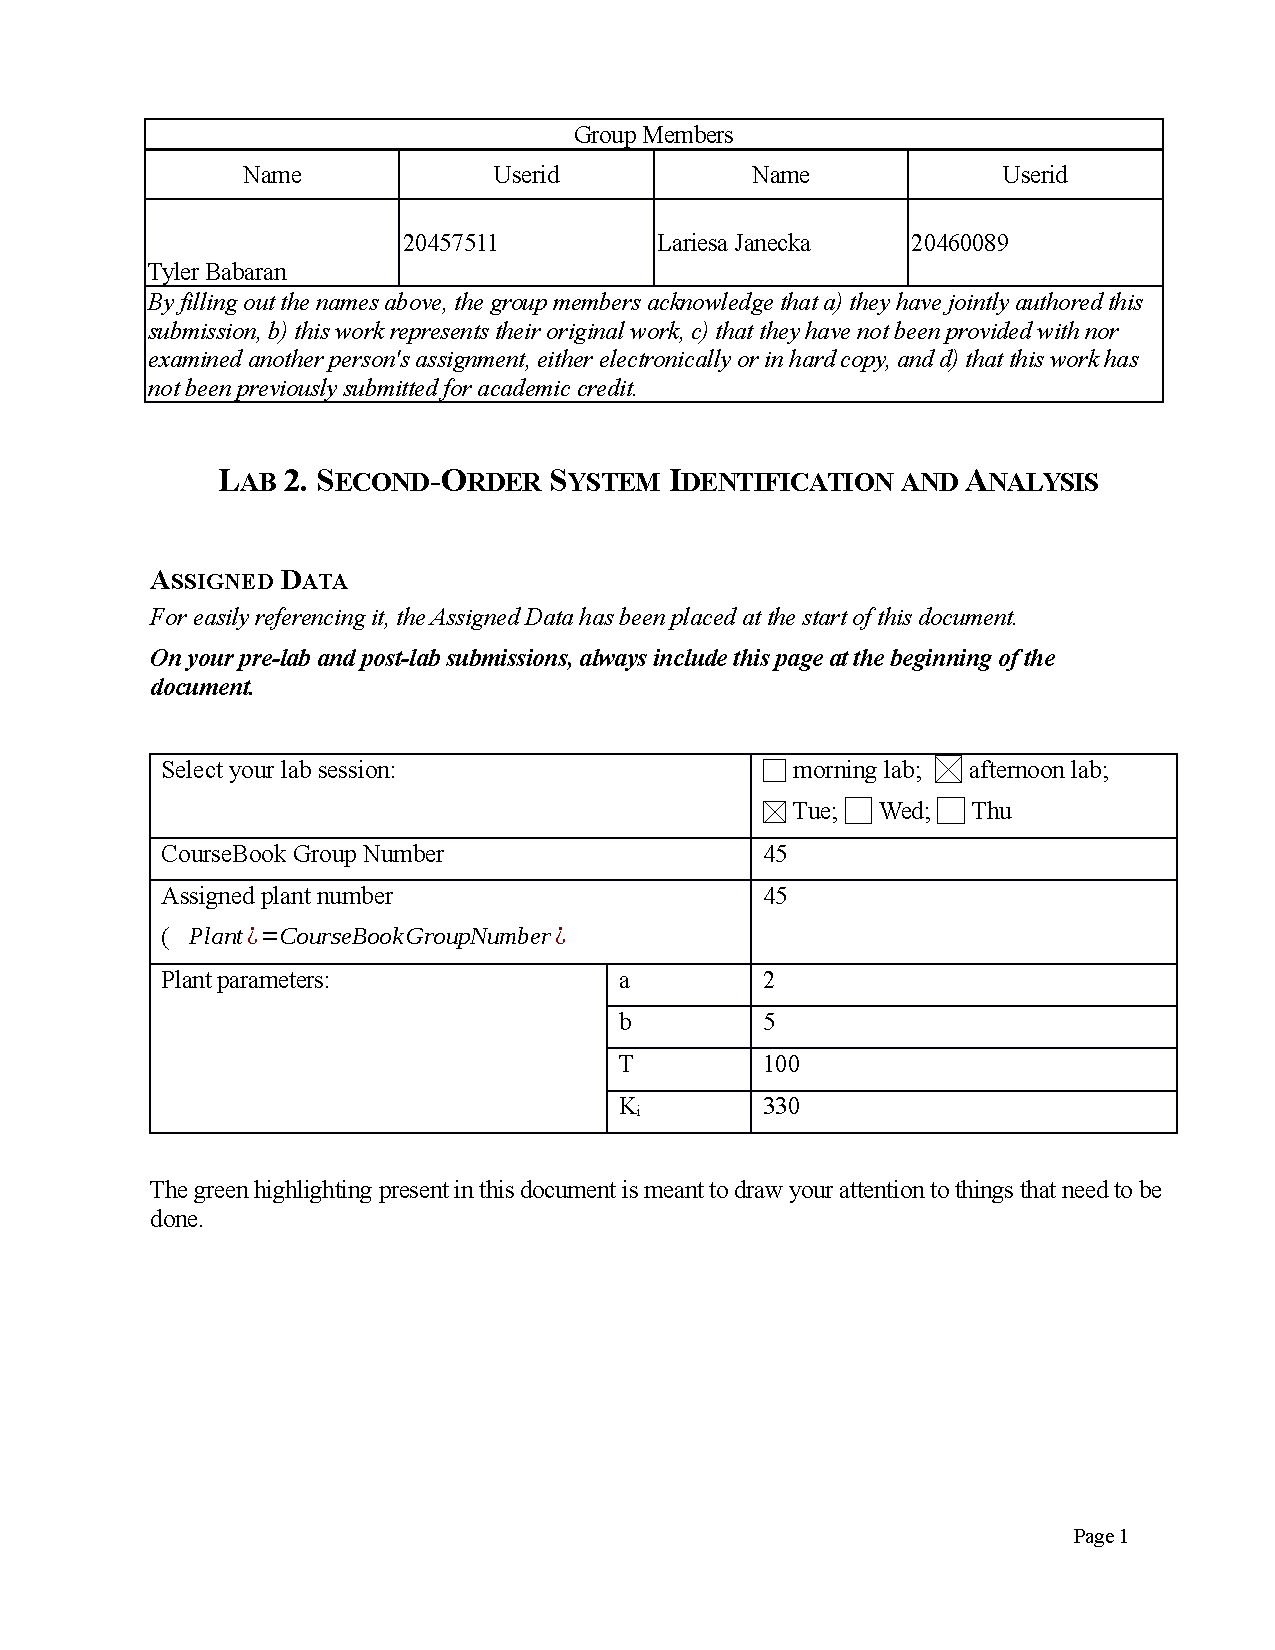
\includepdf[pages={1}]{page1.pdf}
\section*{Section 4.1} % (fold)
\label{sec:section_4_1}
\begin{table}[!htbp]
\centering
    \begin{tabular}{|c|c|c|c|c|}
        \hline
        $T_p$(s) & $c_{max}$ (V) & $c_{ss}$(V) & $T_r$(s) & $T_s$(s)\\
        \hline
        8.22E-003 & 1.48 & 1 & 3.01E-003 & 3.364E-002\\
        \hline
    \end{tabular}
    \caption{Response specifications - experimental values}
\end{table}
\begin{figure}[!htbp]
\centering
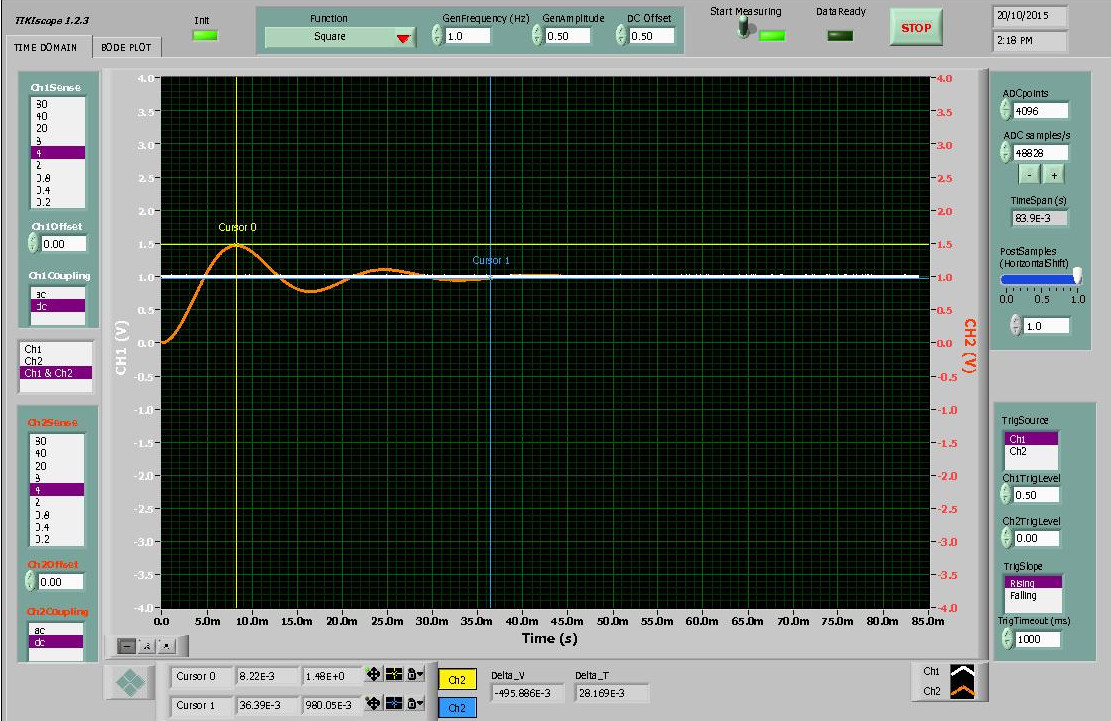
\includegraphics[width=7in]{4_1.jpg}
\caption{Second order underdamped}
\end{figure}
\begin{table}[!htbp]
\centering
    \begin{tabular}{|c|c|c|c|c|c|}
        \hline
        $T_p$(s) & $c_{max}$ (V) & $c_{ss}$(V) & OS(\%) & $\zeta$ & $\omega_n$(rad/s)\\
        \hline
        8.22E-003 & 1.48 & 1 & 48 & 0.2275 & 435.68\\
        \hline
    \end{tabular}
    \caption{System identification data and results}
\end{table}
\newpage

Calculations for table 2:

Using the formula for overshoot
\begin{align*}
    OS &= e^{\frac{-\zeta\pi}{\sqrt{1-\zeta^2}}}\\
    0.48 &= e^{\frac{-\zeta\pi}{\sqrt{1-\zeta^2}}}\\
    \ln {0.48} &= \frac{-\zeta\pi}{\sqrt{1-\zeta^2}}\\
    \ln^2 {0.48} &= \frac{\zeta^2\pi^2}{1-\zeta^2}\\
    \ln^2 {0.48} \times (1-\zeta^2) &= \zeta^2\pi^2\\
    \ln^2 {0.48} &= \zeta^2 \times (\pi^2 +\ln^2 {0.48}) \\
    \zeta &= \sqrt{\frac{\ln^2 {0.48}}{\pi^2 +\ln^2 {0.48}}} \\
    \zeta &=  0.2275\\
\end{align*}

Using the formula for peak time
\begin{align*}
    T_p &= \frac{\pi}{\omega_n\sqrt{1-\zeta^2}}\\
    \omega_n &= \frac{\pi}{T_p\sqrt{1-\zeta^2}}\\
    \omega_n &= \frac{\pi}{0.00822\sqrt{1-\zeta^2}}\\
    \omega_n &= \frac{382.93}{\sqrt{1-\zeta^2}}\\
    \omega_n &= \frac{382.93}{\sqrt{1-0.2275}}\\
    \omega_n &= 435.68\\
\end{align*}


\textbf{Discussing Table 2}

Prelab values: $\zeta = 0.2462$ $\omega = 406.20$

Experimental values: $\zeta = 0.2275$ $\omega = 435.68$

The experimental values differed from the theoretical values calculated in the prelab by around 8\%. Errors may have stemmed from inaccurate graph reading when recording experimental values, or by small rounding errors during mathematical calculations for experimental and theoretical values.

% section section_4_1 (end)
\newpage
\section*{Section 4.2} % (fold)
\label{sec:section_4_2}
\begin{figure}[!htbp]
\centering
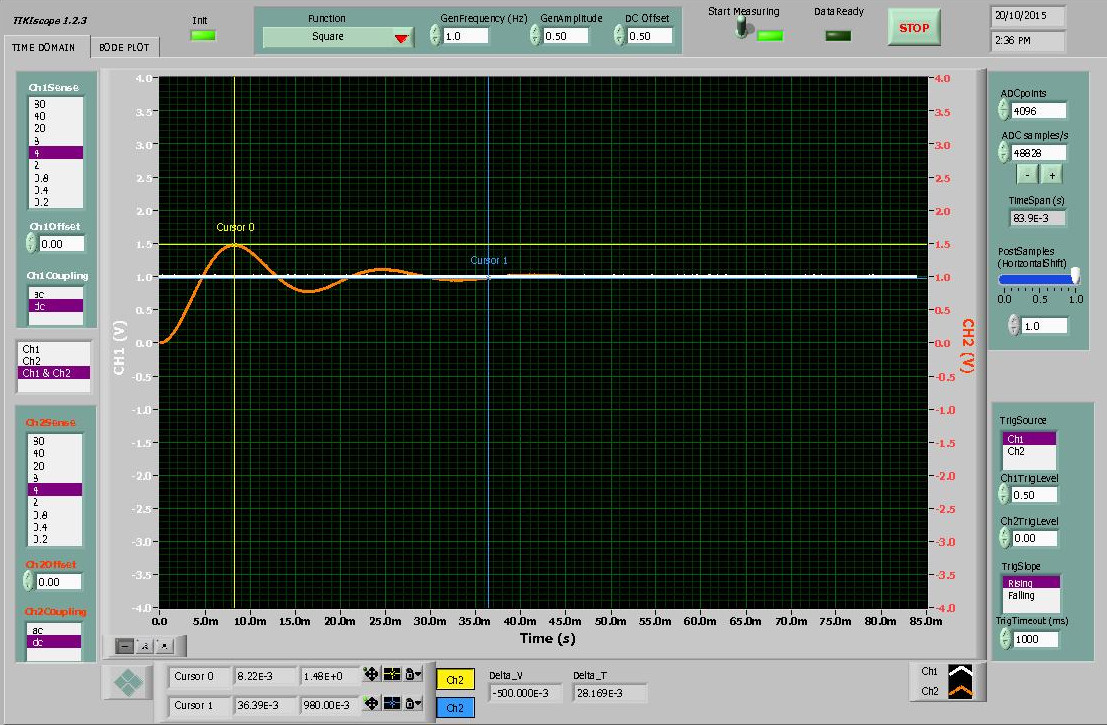
\includegraphics[width=7in]{4_2.jpg}
\caption{Open-loop step response with K=1}
\end{figure}
\begin{table}[!htbp]
\centering
    \begin{tabular}{|c|c|c|c|c|}
        \hline
        $K_p$ & $T_p$(s) & $y_{max}$(V) & $y_{ss}$(V) & OS(\%)\\
        \hline
        1 &8.2E-003 & 1.48 & 1 & 48\\
        \hline
        1.3 & 8.17E-003 & 1.98 & 1.33 & 49\\
        \hline
        1.66 & 8.27E-003 & 2.47 & 1.66 & 49\\
        \hline
        2 &8.17E-003 & 2.93 & 2 & 47\\
        \hline
    \end{tabular}
    \caption{Open-loop step response values for Kp=variable}
\end{table}
\newpage

\textbf{Discussing Table 3}

\textbf{Peak Value}: This increased with Kp. This fits control theory as the peak value is the highest oscillation above the steady state value, since the steady state value is increasing without $\zeta$ changing this value should rise as well.

\textbf{Steady state}: As Kp increases the steady state value increases to match the Kp value. This fits with control theory as the output for G(S) has a steady state value of 1, experimentally verified. For the open loop system the output should be equal to $G(S)\times K\times K_p$ (as they are all in series) and since K stayed at 1 for all experiments the output increase was proportional to Kp.

\textbf{Overshoot and Peak time}: These values did not change much. This fits control theory as the equations for overshoot and peak time are proportional to $\zeta$ and $\omega_n$ which do not vary with with K or Kp in the open-loop system.

\begin{figure}[!htbp]
\centering
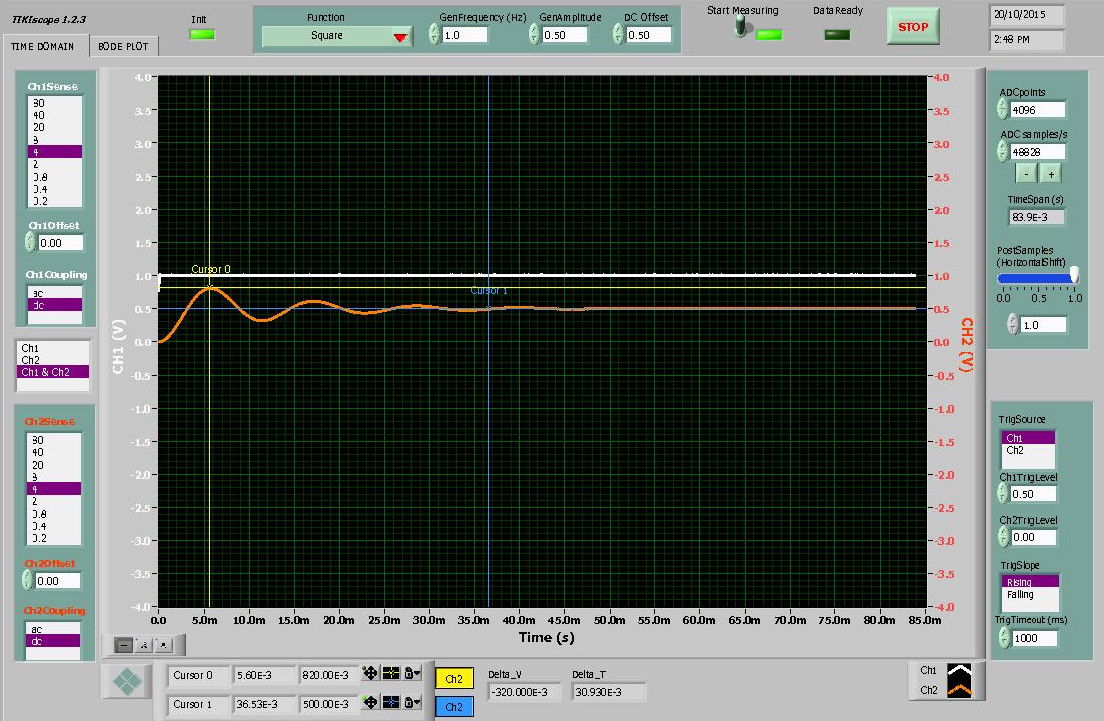
\includegraphics[width=7in]{4_2b.jpg}
\caption{Closed-loop step response with K=1}
\end{figure}
\begin{table}[!htbp]
\centering
    \begin{tabular}{|c|c|c|c|c|c|}
        \hline
        $K_p$ & $T_p$(s) & $y_{max}$(V) & $y_{ss}$(V) & $e_{ss}$ & OS(\%)\\
        \hline
        1 & 5.6E-003 & 0.82 & 0.5 & 0.5 & 64\\
        \hline
        1.3 & 5.2E-003 & 0.93 & 0.57 & 0.565 & 63\\
        \hline
        1.66 & 4.92E-003 & 1.03 & 0.64 & 0.615 & 62\\
        \hline
        2 & 4.5E-003 & 1.12 & 0.68 & 0.667 & 65\\
        \hline
    \end{tabular}
    \caption{Closed-loop step response values for Kp=variable}
\end{table}

\textbf{Discussing Table 4}

\textbf{Peak Value and Steady State value}: These values are increasing with Kp. Due to control theory our system output with the increase of Kp from 1 is:
\begin{align*}
      Y(S) = \frac{K_pH(S)}{1 + K_pH(S)}
  \end{align*}
As Kp increases in the above equation the output will also increase is what causes the increase in the peak value and the steady state value.

\textbf{Overshoot}: The overshoot does not change much. This is due to the steady state and peak value increasing by the same ratio. We can also see that this value will not change because it is related to $\zeta$ which has not changed.

\textbf{Peak Time}: The peak time is decreasing as Kp increases. This is due to the peak time being inversely proportional to the natural frequency. In this system the natural frequency was proportional to Kp, so when Kp increases the natural frequency increases which causes the peak time to decrease.

\textbf{Zeta and Omega Calculations}

The new transfer function for the system is:
\begin{align*}
    H(S) &= \frac{K_ibTKK_p}{s^2 + aTs + K_ibT + K_ibTK_pK}\\
            & K_p = 1 \tt{ and } K = 1\\
            &= \frac{K_ibT}{s^2 + aTs + 2K_ibT}\\
            &= \frac{1}{2} \times \frac{2K_ibT}{s^2 + aTs + 2K_ibT}\\
\end{align*}
This is a standard second order system with a coefficient. Since coefficients carry over during a Laplace transform we can use the equations for a standard second order system with the coefficient.

Based on the definition of standard second order system:
\begin{align*}
    \omega_n^2 &= 2K_ibTKK_p\\
    \omega_n &= \sqrt{2K_ibTKK_p}\\
        &= \sqrt{2 * 330 * 5 * 100}\\
        &= \sqrt{2 * 330 * 5 * 100}\\
        &= 574.45
\end{align*}
\begin{align*}
    aT &= 2\zeta\omega_n\\
    \zeta &= \frac{aT}{2\omega_n}\\
        &= \frac{2 * 100}{2 * 574.45}\\
        &= 0.35
\end{align*}


Using the formula for overshoot
\begin{align*}
    OS &= \frac{1}{2} e^{\frac{-\zeta\pi}{\sqrt{1-\zeta^2}}}\\
    \zeta &= \sqrt{\frac{\ln^2 {\frac{OS}{2}}}{\pi^2 +\ln^2 {\frac{OS}{2}}}} \\
    \zeta &= \sqrt{\frac{\ln^2 {\frac{0.64}{2}}}{\pi^2 +\ln^2 {\frac{0.64}{2}}}} \\
    \zeta &=  0.34\\
\end{align*}

Since the peak time formula is found by taking the sinusoidal function is highest, it is not influenced by the added coefficient so we can use the same function for calculating $\omega_n$.
Using the formula for peak time
\begin{align*}
    T_p &= \frac{\pi}{\omega_n\sqrt{1-\zeta^2}}\\
    \omega_n &= \frac{\pi}{T_p\sqrt{1-\zeta^2}}\\
    \omega_n &= \frac{\pi}{0.0056\sqrt{1-0.34^2}}\\
    \omega_n &= 596.76\\
\end{align*}


Experimental Open-loop: $\zeta = 0.2275$ $\omega_n = 435.68$

Experimental Closed-loop: $\zeta = 0.34$ $\omega_n = 596.76$

Theoretical Open-loop: $\zeta = 0.2462$ $\omega = 406.20$

Theoretical Closed-loop: $\zeta = 0.35$ $\omega_n = 575.45$

The dampening ratio increased when the loop was closed due to the stabilizing nature of a closed loop. The output is dampened by the subtraction of itself from the input. The transfer function multiplied to natural frequency by 2 which resulted in it increasing by a factor of $\sqrt{2}$.


Adjusted value is k=1.04

\begin{table}[!htbp]
\centering
    \begin{tabular}{|c|c|c|c|c|}
        \hline
        & Low-freq gain (dB) & Experimental bw (rad/s) & Theor or sim bw (rad/s) & Error (\%)\\
        \hline
        Open-loop & 0.5 & 589 & 603 & 2.4\\
        \hline
        Closed-loop & -5.8 & 850 & 869 & 2.2\\
        \hline
    \end{tabular}
    \caption{Bandwidth (bw) measurement results}
\end{table}
Closing the loop dramatically increased the measured bandwidth. Bandwidth is defined as the range of frequencies over which the output is is relatively close to the input. We want to be able to change bandwidth in order to lessen the amount of disturbance.

\begin{figure}[!htbp]
\centering
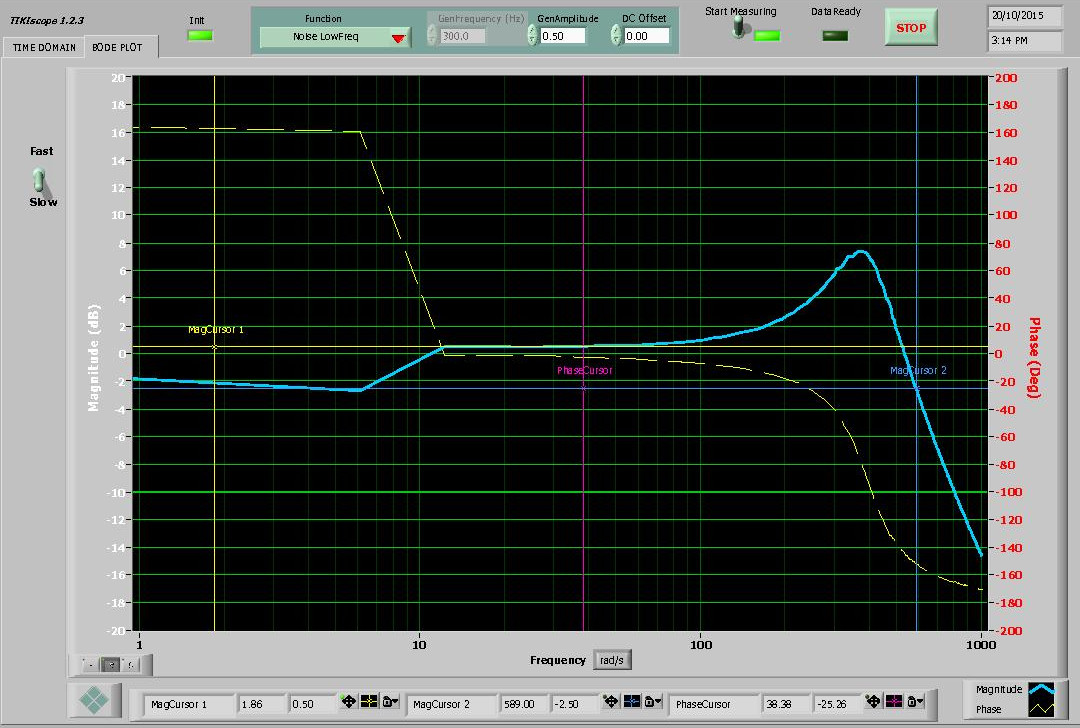
\includegraphics[width=7in]{4_2c(open).jpg}
\caption{Open-loop frequency response}
\end{figure}

\begin{figure}[!htbp]
\centering
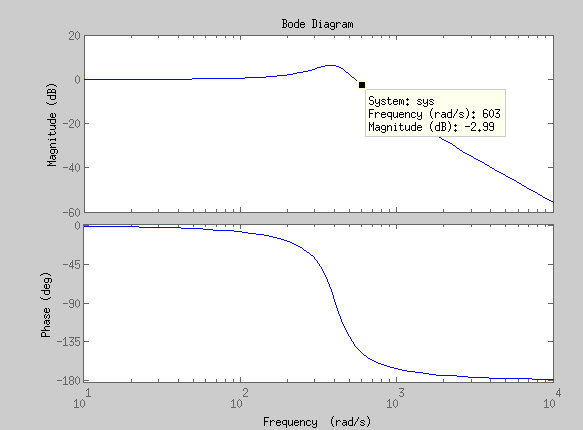
\includegraphics[width=7in]{4_2c(open)_matlab.png}
\caption{Matlab open-loop frequency response}
\end{figure}

\begin{figure}[!htbp]
\centering
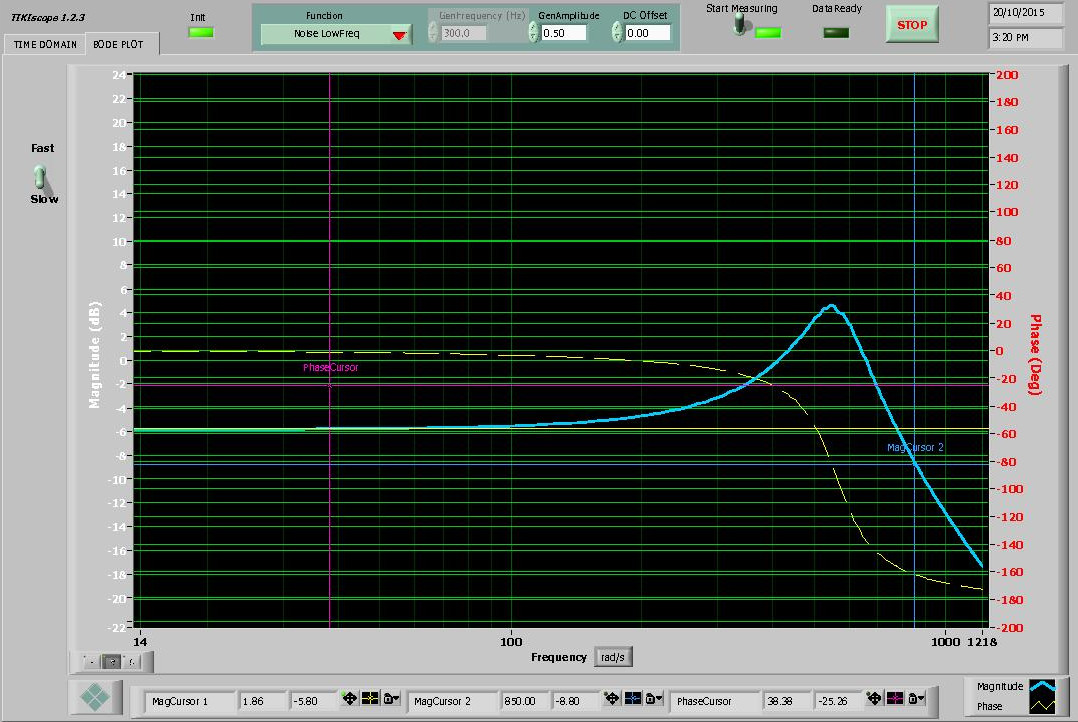
\includegraphics[width=7in]{4_2c(closed).jpg}
\caption{Closed-loop frequency response}
\end{figure}

\begin{figure}[!htbp]
\centering
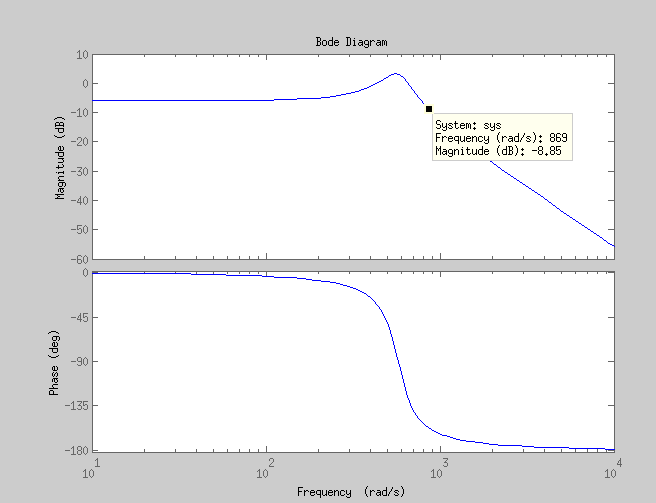
\includegraphics[width=7in]{4_2c(closed)_matlab.png}
\caption{Matlab closed-loop frequency response}
\end{figure}

% section section_4_2 (end)
\newpage
\section*{Section 4.3} % (fold)
\label{sec:section_4_3}
\begin{figure}
\centering
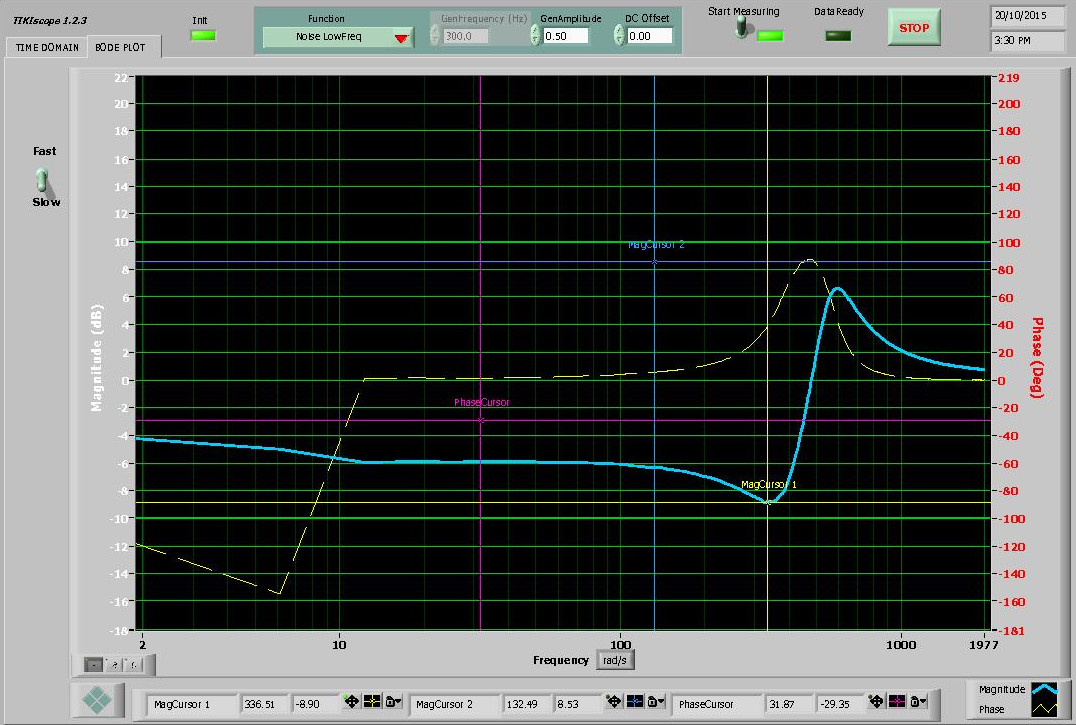
\includegraphics[width=7in]{4_3.jpg}
\caption{Frequency response response with disturbance}
\end{figure}
The equation for the system with input at D(S) is:

As shown in Figure 8 frequencies below 336.51 rad/s show little disturbance and frequencies after that show wild changes in response to the disturbances.

In the open-loop system there is no disturbance rejection since nothing is piped back in. The disturbance is directly added to our output. Due to the closed nature of the closed-loop system there is disturbance rejection by subtracting the output from the input.
% section section_4_3 (end)



\end{document}




